% fig18-tactic-roles.tex
% Absorbed vs load-bearing tactic roles under intervention
\documentclass[tikz,border=18pt]{standalone}
% common-styles.tex
% Shared TikZ styles for wonton-proof paper figures

\usepackage{silence}
\WarningFilter{latex}{Missing character} 
\tracinglostchars=0 % Suppress engine-level "Missing character" warnings

\usepackage{fontspec}
\usepackage{unicode-math}

% Use filenames for reliability with Tectonic
\setmainfont{LibertinusSerif-Regular.otf}[
    BoldFont=LibertinusSerif-Bold.otf,
    ItalicFont=LibertinusSerif-Italic.otf,
    BoldItalicFont=LibertinusSerif-BoldItalic.otf
]
\setsansfont{LibertinusSans-Regular.otf}[
    BoldFont=LibertinusSans-Bold.otf,
    ItalicFont=LibertinusSans-Italic.otf
]
\setmonofont{LibertinusMono-Regular.otf}

% Try a more standard math font if LibertinusMath is causing nullfont issues
\setmathfont{LibertinusMath-Regular.otf}
% \setmathfont{latinmodern-math.otf}[range=digits] 

\usepackage{amsmath}
\usepackage{tikz}
\usepackage{forest}

\usetikzlibrary{
    arrows.meta,
    calc,
    decorations.pathreplacing,
    fit,
    positioning,
    shapes.geometric,
    shapes.misc,
    backgrounds,
    shadows.blur,
    fadings
}

% Color palette (muted, print-friendly)
\definecolor{ink}{RGB}{45,45,52}
\definecolor{muted}{RGB}{115,115,125}
\definecolor{highlight}{RGB}{198,120,44}
\definecolor{accentblue}{RGB}{86,130,178}
\definecolor{accentgreen}{RGB}{84,156,132}
\definecolor{blocked}{RGB}{140,75,75}
\definecolor{goalnode}{RGB}{255,255,255}
\definecolor{terminal}{RGB}{238,239,244}
\definecolor{deadnode}{RGB}{248,245,245}
\definecolor{flowbox}{RGB}{250,250,252}
\definecolor{basin1}{RGB}{224,234,248}
\definecolor{basin2}{RGB}{246,232,221}
\definecolor{basin3}{RGB}{228,242,234}
\definecolor{heatbase}{RGB}{86,130,178}

\tikzset{
    line cap=round,
    line join=round,
    pop/.style={
        blur shadow={shadow blur steps=5, shadow blur extra rounding=1.3pt}
    },
    base node/.style={
        rounded rectangle,
        draw=ink,
        line width=0.6pt,
        fill=goalnode,
        text=ink,
        minimum width=2.2cm,
        minimum height=0.7cm,
        align=center,
        pop
    },
    goal/.style={base node, fill=goalnode},
    terminal/.style={base node, fill=terminal, line width=0.9pt},
    dead/.style={base node, fill=deadnode, dashed},
    flowbox/.style={
        rectangle,
        draw=muted,
        rounded corners=3pt,
        fill=flowbox,
        minimum width=1.8cm,
        minimum height=0.6cm,
        align=center,
        font=\normalfont\small,
        text=ink,
        pop
    },
    decision/.style={
        diamond,
        draw=muted,
        fill=flowbox,
        aspect=2.4,
        font=\normalfont\small,
        inner sep=1pt,
        text=ink
    },
    protocolbox/.style={
        rectangle,
        draw=muted,
        rounded corners=4pt,
        fill=flowbox,
        minimum width=2cm,
        minimum height=0.8cm,
        font=\normalfont\small,
        align=center,
        text=ink
    },
    tactic/.style={
        ->,
        >=Stealth,
        draw=muted,
        line width=0.75pt
    },
    tacticlight/.style={
        ->,
        >=Stealth,
        draw=muted!45,
        dashed,
        line width=0.6pt
    },
    backprop/.style={
        ->,
        >=Stealth,
        draw=muted!70,
        dashed,
        line width=0.6pt
    },
    selected/.style={
        tactic,
        draw=highlight,
        line width=1.4pt
    },
    divergetactic/.style={
        tactic,
        draw=highlight,
        line width=1.4pt
    },
    divergenode/.style={
        base node,
        draw=highlight,
        line width=1.0pt
    },
    divergeblock/.style={
        blockedtactic,
        line width=1.2pt
    },
    blockedtactic/.style={
        tactic,
        draw=blocked,
        densely dashed
    },
    flowarrow/.style={
        ->,
        >=Stealth,
        draw=muted,
        line width=0.75pt
    },
    crosslink/.style={
        -,
        draw=muted!70,
        dotted,
        line width=0.6pt
    },
    annot/.style={
        font=\normalfont\footnotesize,
        text=muted
    },
    visit/.style={
        annot,
        font=\normalfont\scriptsize
    },
    annotbg/.style={
        annot,
        fill=white,
        inner sep=1.5pt
    },
    tacticlabel/.style={
        annot,
        font=\ttfamily\footnotesize,
        text=muted
    },
    formula/.style={
        font=\normalfont\footnotesize,
        draw=muted,
        rounded corners=2pt,
        fill=white,
        inner sep=3pt
    },
    paneltitle/.style={
        font=\normalfont\bfseries,
        text=ink
    },
    trajectory/.style={
        ->,
        draw=muted!70,
        line width=0.6pt
    }
}


\begin{document}
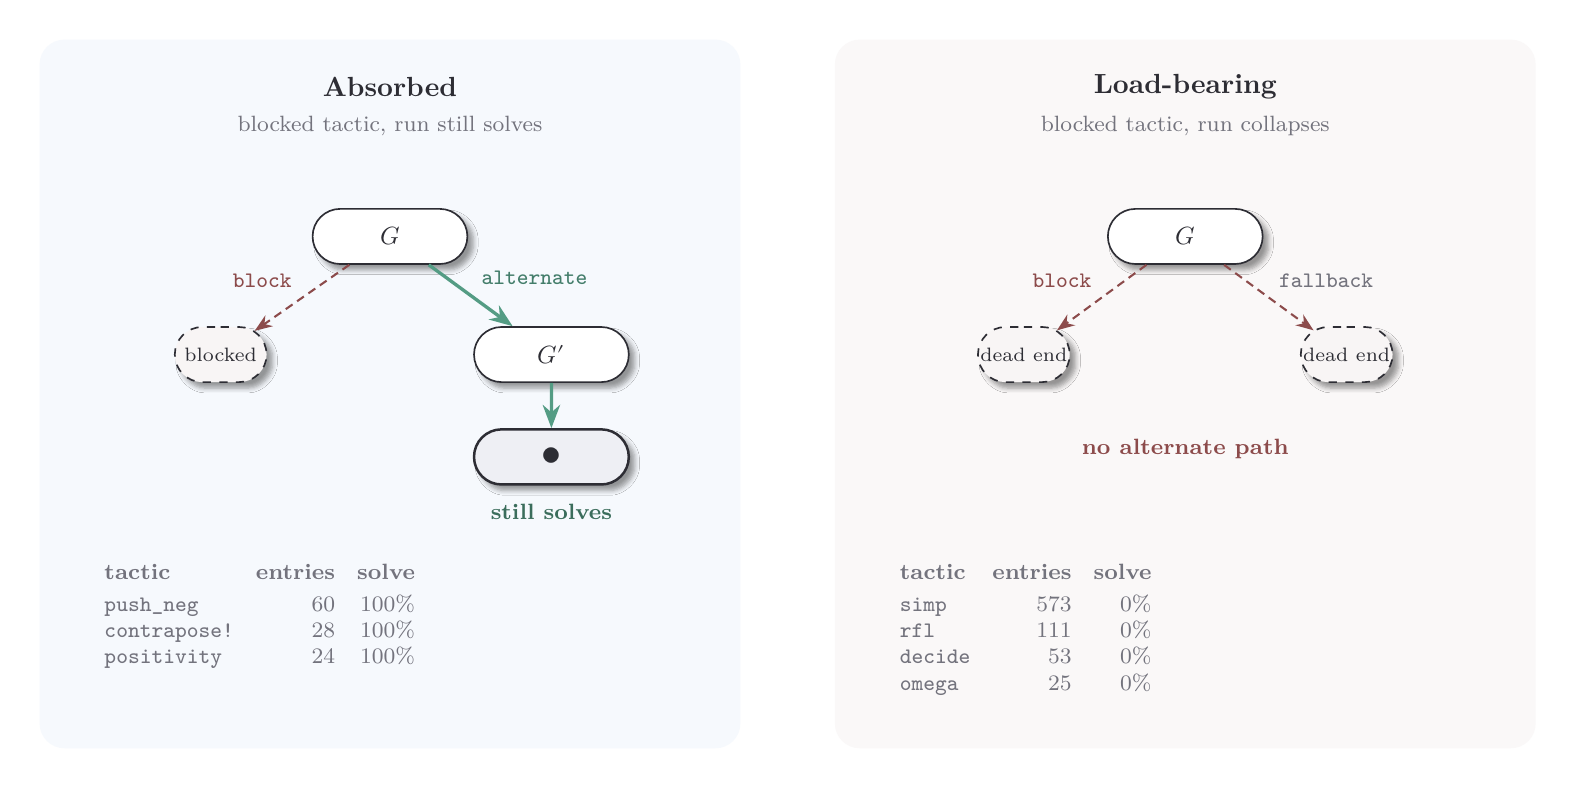
\begin{tikzpicture}[
    every node/.style={font=\small},
    show background rectangle,
    background rectangle/.style={fill=white}
]

% Background panels
\path[fill=basin1!28, rounded corners=9pt] (-9.5, -4.5) rectangle (-0.6, 4.5);
\path[fill=deadnode!70, rounded corners=9pt] (0.6, -4.5) rectangle (9.5, 4.5);

% === LEFT PANEL: Absorbed ===
\node[paneltitle] at (-5.05, 3.9) {Absorbed};
\node[annot] at (-5.05, 3.4) {blocked tactic, run still solves};

% Schematic: blocked path + green success path
\node[goal] (al0) at (-5.05, 2.0) {$G$};
\node[dead, minimum width=1.4cm] (ald) at (-7.2, 0.5) {\scriptsize blocked};
\node[goal] (al1) at (-3.0, 0.5) {$G'$};
\node[terminal] (alt) at (-3.0, -0.8) {{\Large$\bullet$}};

\draw[blockedtactic] (al0) -- (ald)
    node[midway, above left, tacticlabel, text=blocked] {block};
\draw[tactic, draw=accentgreen, line width=1.2pt] (al0) -- (al1)
    node[midway, above right, tacticlabel, text=accentgreen!80!black] {alternate};
\draw[tactic, draw=accentgreen, line width=1.2pt] (al1) -- (alt);

\node[annot, text=accentgreen!70!black, font=\normalfont\footnotesize\bfseries]
    at (-3.0, -1.5) {still solves};

% Tactic list with solve rates
\node[annot, anchor=north west, align=left, font=\normalfont\footnotesize]
    at (-8.8, -2.0) {%
        \begin{tabular}{@{}l@{\quad}r@{\quad}r@{}}
        \textbf{tactic} & \textbf{entries} & \textbf{solve} \\[2pt]
        \texttt{push\_neg} & 60 & 100\% \\
        \texttt{contrapose!} & 28 & 100\% \\
        \texttt{positivity} & 24 & 100\% \\
        \end{tabular}%
    };

% === RIGHT PANEL: Load-bearing ===
\node[paneltitle] at (5.05, 3.9) {Load-bearing};
\node[annot] at (5.05, 3.4) {blocked tactic, run collapses};

% Schematic: blocked path leads to dead ends
\node[goal] (bl0) at (5.05, 2.0) {$G$};
\node[dead, minimum width=1.4cm] (bld1) at (3.0, 0.5) {\scriptsize dead end};
\node[dead, minimum width=1.4cm] (bld2) at (7.1, 0.5) {\scriptsize dead end};

\draw[blockedtactic] (bl0) -- (bld1)
    node[midway, above left, tacticlabel, text=blocked] {block};
\draw[blockedtactic] (bl0) -- (bld2)
    node[midway, above right, tacticlabel, text=muted] {fallback};

\node[annot, text=blocked, font=\normalfont\footnotesize\bfseries]
    at (5.05, -0.7) {no alternate path};

% Tactic list with solve rates
\node[annot, anchor=north west, align=left, font=\normalfont\footnotesize]
    at (1.3, -2.0) {%
        \begin{tabular}{@{}l@{\quad}r@{\quad}r@{}}
        \textbf{tactic} & \textbf{entries} & \textbf{solve} \\[2pt]
        \texttt{simp} & 573 & 0\% \\
        \texttt{rfl} & 111 & 0\% \\
        \texttt{decide} & 53 & 0\% \\
        \texttt{omega} & 25 & 0\% \\
        \end{tabular}%
    };

\end{tikzpicture}
\end{document}
